\section{Resisitive switch design}
\label{sec:resisitive_switch_design}
This chapter will show the theoretical concepts and propose a design of a cantilever based micro-switch.
Trade-offs and important parameters will be explained.
Also all simplifications are described here.

\subsection{Contact}
\label{sec:contact}
Optimized contact pads have serious constraints on geometry, materials, contact force and release force. 
Due to the small scope of this project the contact pads were not further studied and were defined as being of a simple rectangular shape.
The material was chosen to be gold for it's good electric and mechanical properties. 

A choice was made between two designs.
The first possibility was to use a cantilever with a single contact point, so that the current would flow through the cantilever itself. %image
The second possibility was to use a cantilever with a simple golden surface, that would connect two fixed contact points to one another. %image
The second design was chosen to guarantee a small lenght of the contact element and therefore to reduce it's resistance and power consumption.
Also the mechanical properties of the cantilever don't get influenced that heavily by the second choice and therefore enables the design, of all but the tip of the cantilever, to focus on the actuation and guidance functionality of the structure.
The disadvantage of this design choice is a minimum required width, which is given by the resolution of the fabrication process of two non-connected pads.

\subsection{Actuation}
\label{sec:actuation}
There are four different actuation principles which can be used for a mechanical micro-switch design:
\begin{itemize}
  \item Electrostatic
  \item Piezoelectric
  \item Electromagnetic
  \item Thermal
\end{itemize}

Thermal actuators are not fast enough for micro-switch applications. 
Also they have the highest power consumption of all the methods.

Electromagnetic actuators require either a permanent magnetic material or an electromagnet design to work.
The material choices are therefore difficult and also the footprint would be rather big compared to the other methods.

Piezoelectric actuators represent the method with the lowest power consumption.
But compared to electrostatic actuators they are way more complex to fabricate and material choices represent a challenge.\cite{klaasse2002piezoelectric}

Therefore our choice fell on an electrostatic actuator.
They are very simple from a fabrication point of view, allow low power consumption and offer a fast actuation time.

\subsection{Basic Concepts}
\label{sec:basic_concepts}

Our switch design is based on a beam cantilever, so we start with the deflection of a clamped beam with a force applied at an arbitrary point along the beam (\ref{eq:beam_deflection}).

\begin{equation}
    \delta(x) = \begin{cases} \frac{Fx^2}{6EI_z} \cdot (3a-x) & \mbox{for } 0 < x < a \\
                              \frac{Fa^2}{6EI_z} \cdot (3x-a) & \mbox{for } a < x < l
                \end{cases}
    \label{eq:beam_deflection}
\end{equation}


With the area moment of inertia defined as such:
\begin{equation}
	I_z = \frac{wt^3}{12}
	\label{eq:area_moment_of_inertia}
\end{equation}

and the distance $a$ like it is shown in Figure~\ref{fig:cantilever_beam}.

\begin{figure}[h]
	\centering
	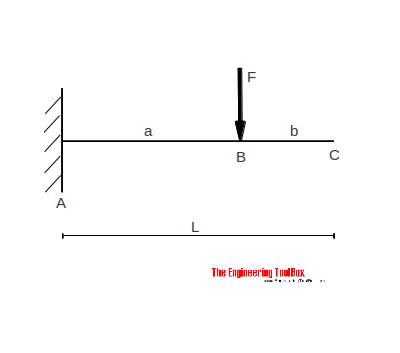
\includegraphics[width=8cm]{fig/cantilever_beam_single_load.png}
    \caption{Clamped beam with a single load.}
\label{fig:cantilever_beam}
\end{figure}

\subsubsection{Resonance frequency}
In order to estimate the time it takes to flip the switch, we calculate the \emph{resonance frequency} of the beam.
We can simplify the cantilever as a harmonic oscillator (mass-spring).
In that case we calculate the resonance frequency using equation (\ref{eq:resonance_frequency}).

\begin{equation}
	\omega_0 = \sqrt{\frac{k}{m_{eff}}}
	\label{eq:resonance_frequency}
\end{equation}

We need to calculate the spring constant $k$ and the effective mass $m_{eff}$ of the beam.
From (\ref{eq:beam_deflection}) we can conclude (\ref{eq:spring_constant}) for the spring constant.

\begin{equation}
	k = \frac{F}{\delta} = \frac{6EI_z}{a^2(3l-a)}
	\label{eq:spring_constant}
\end{equation}

Equation (\ref{eq:effective_mass}) defines the effective mass~\cite{wong2011theoretical}.

\begin{equation}
	m_{eff} = \rho A \int_0^l{\left[\frac{\delta(x)}{\delta(l)_{max}}\right]^2dx}
	\label{eq:effective_mass}
\end{equation}

If we evaluate (\ref{eq:effective_mass}) for a beam with the force applied at the extremity, we get $m_{eff} = 33/140 m$.
When we apply the force at an arbitrary position $a$, the expression becomes $m_{eff} = \frac{6l^2-4al+a^2}{12l^2-4al} m$.
If we choose a value for $a$ more or less close to $l$, we can just use $33/140m$ for simplicity.


\subsubsection{Electrostatic force}
Equation (\ref{eq:electrostatic_force}) gives the electrostatic force between two metal plates.
One notes that this is neglecting any \emph{fringe effects}.
We can do that when the distance between the plates is much smaller than the side lengths of the plates.

\begin{equation}
	F_{ES} = \frac{\varepsilon AV^2}{2d^2}
	\label{eq:electrostatic_force}
\end{equation}

\subsubsection{Switch resistance}
The resistance of the contact which closes the switch depends on thickness of the metal plating and \emph{aspect ratio} of it's shape, as well as the plated material's resistivity.
\begin{equation}
	R = \rho_{el}\frac{l}{wt}
	\label{eq:resistance}
\end{equation}

\subsubsection{Actuator pad capacitance}
The actuator forms a \emph{capacitor}, which we have to charge when we want to operate the switch.
This charging takes time we have to make sure that it isn't a limiting factor.

Equation (\ref{eq:plate_capacitor}) gives the \emph{capacitance} of the actuator.

\begin{equation}
	C = \frac{\varepsilon A}{d}
	\label{eq:plate_capacitor}
\end{equation}

We then get the time constant $\tau$ in equation (\ref{eq:rc_time_constant}).

\begin{equation}
    \tau = RC
    \label{eq:rc_time_constant}
\end{equation}

With $R$ being the resistance of the circuit charging the capacitor.

\subsubsection{Thermal analysis}

We neglect any thin-film effects and there are no currents expected to be high enough to heat the mechanism up to a point where it starts to matter.


\subsection{Analysis}
\label{sec:analysis}

\subsubsection{Simplifications}
\label{ssub:simplifications}
We identified some things which we could simplify for our analysis:

\paragraph{Fringe effects}
The aspect ratio of our actuator makes it so that the fringe effects are negligible for our electrostatic actuation force.

\paragraph{Actuator capacitance}
In case of the proposed dimensions, the capacitance of the actuator is in the order of pico Farads, which results in cut-off frequencies of more than \SI{1}{\tera\hertz\ohm}.
It's impossible that this frequency would ever be a limiting factor of the switch.

\paragraph{Switch resistance}
With the constraint of \SI{10}{\ohm} of resistance of our switch, we can say that the aspect ratio of the actuation pad has to be better than $43$ (i.e.\ not more than $43$ times longer than wide) when we use a \SI{100}{\nano\meter} thick gold pad.
This should be easily fulfilled with any kind of design that we could come up with.

\paragraph{Effective mass}
The designs that we analysed had the actuation force placed close enough to the free end of the beam so that we could use the simplified expression of the effective mass which supposes the force to be at the very end.


\subsubsection{Optimizations}
\label{ssub:optimizations}

Our goals were:

\begin{itemize}
    \item Short response time
    \item Low activation voltage
    \item Small footprint
\end{itemize}

There are some obvious trade-offs like that switching will always be faster with a higher Force applied to the actuator.
This calls for an as high as possible activation voltage and the smallest possible \emph{air gap}.
When you look at equation (\ref{eq:switching_time_optimization}) you can see that the switching time actually converges when the activation voltage becomes infinity.
So, one could argue that once the total switching time reached a certain percentage of the minimal value, it is inefficient to increase the voltage further.
But with the order of magnitude of our proposed dimensions, this would be in the \SI{}{\kilo\volt} (as opposed to the \SI{10}{\volt} which were imposed as limit).

On the other hand, a small footprint has a positive influence of the response time, because the footprint scales with the square of the length, while the mass scales with the cube, and response time depends on the ratio between mass and length.

The chose the actual shape of the beam by looking at how the spring constant changes.
The Appendix~\ref{appendix} talks at length about how to chose the optimal $k$.
There exists an optimum, but we can't calculate it analytically.

\subsubsection{Proposed dimensions}
\label{ssub:proposed_dimensions}

Doing the above mentioned simplifications, optimizations, and trade-offs, we came to propose a cantilever as shown in Figure~\ref{fig:cantilever_design} with silicon as the structural material and gold for the contact pads (Table~\ref{tab:silicium_mat}~\&~\ref{tab:gold_mat} contain their properties).
With an activation voltage of \SI{10}{\volt} we reach switching frequencies of dozens of \SI{}{\mega\hertz} with contact forces of dozens of \SI{}{\milli\newton}.


\begin{figure}[h]
	\centering
	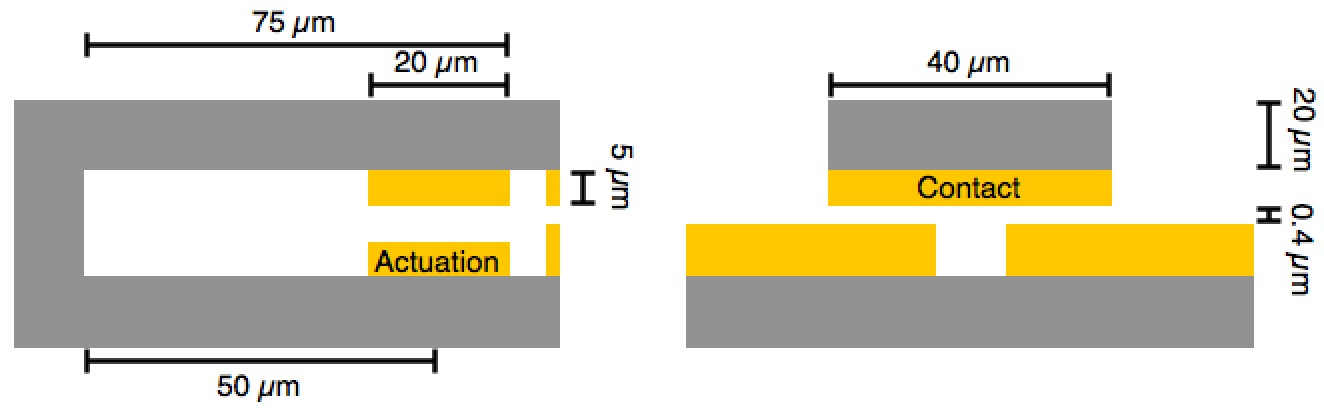
\includegraphics[width=12cm]{fig/cant_design.jpg}
    \caption{Cantilever design with dimensions.}
\label{fig:cantilever_design}
\end{figure}

\begin{table}
	\centering
	\begin{tabular}{l l r l} 
		\toprule
		Property & symbol & Value & Unit \\
		\midrule
		Density & $\rho$ & 2.329 & $g/cm^3$ \\
		Young's Modulus & E & 186.5 & GPa \\ 
		Poisson's Ratio & $\upsilon$ & 0.25 & - \\ 
		Dielectic Constant & $\epsilon_r$ & 11.9 & - \\
		Resistivity & $\rho_{el}$ & $3.2\cdot10^5 $ & $\Omega \cdot cm$ \\
		\bottomrule
	\end{tabular}
	\caption{Material properties of [111] silicon}
	\label{tab:silicium_mat}
\end{table}

\begin{table}[H]
	\centering
	\begin{tabular}{l l r l} 
		\toprule
		Property & symbol & Value & Unit \\
		\midrule
		Density & $\rho$ & 19.30 & $g/cm^3$ \\
		Young's Modulus & E & 79 & GPa \\ 
		Poisson's Ratio & $\upsilon$ & 0.4 & - \\ 
		Dielectic Constant & $\epsilon_r$ & 6.9 & - \\
		Resistivity & $\rho_{el}$ & $22.14\cdot10^{-9} $ & $\Omega \cdot cm$ \\
		\bottomrule
	\end{tabular}
	\caption{Material properties of Gold}
	\label{tab:gold_mat}
\end{table}
